\subsubsection{求解与结果分析：碳化硅厚度及双角核对}

共享厚度与逐角低阶响应分开后，求解的重点便是交出厚度，并检查这个数能否解释未参与拟合的光谱。这里先报告同片结果，再用连续留段和双向留角度核对条纹。

碳化硅外延层的同片非触边代表厚度为$10.80\ \mu\mathrm{m}$，厚度重估范围为$0.64$--$18.11\ \mu\mathrm{m}$。点值对应透明两束、经验色散及逐角低阶响应；范围则记录搜索、切分和光学条件变化带来的厚度移动。表\ref{tab:q2-results}将计算设置、同片代表值与分项核对并列，两个附件共同决定厚度，而非分别求厚后取平均。
% src:求解/问题2/结果/厚度结果.json:同片最佳厚度_微米;条件区间_微米;光学情景;输入附件

这里采用的是固定比较基准的规则，而非加密后重新选优：在原厚度网格$96$点搜索内取最低损失可行解，各参数距上下界的距离除以搜索跨度后均须大于$10^{-4}$。原点的最小相对边界距离为$0.0610$，满足该规则；表\ref{tab:q2-search-check}中的加密触边候选仍参与全部候选的损失比较，不因触边而被排除。
% src:求解/问题2/结果/搜索补查.json:代表点规则;候选.0.最小相对边界距离

按训练损失排序，现有补查最低的厚度是$13.53\ \mu\mathrm{m}$，不是沿用的$10.80\ \mu\mathrm{m}$。前者折射率触及搜索下界，后者承担跨问题比较坐标；这两个身份分列，搜索产生的分支差异也与改变光学假设的情景差异分别讨论。厚度保留两位小数是报告格式，测量精度仍受光学假设和取段变化限制。
% src:求解/问题2/结果/搜索补查.json:候选.0.厚度_微米;补查最低损失候选.厚度_微米;补查最低损失候选.触边参数

附件一（十度）与附件二（十五度）在共同原始坐标上同步抽样。给定厚度与折射变化后，先直接求出各角基线和幅值，再作多起点有界搜索；这种安排把条纹位置留给共享参数，把角度造成的包络差别交给低阶响应。连续块承担训练、校准和测试的不同任务，训练边界另留$20\ \mathrm{cm}^{-1}$保护带，避免相邻波数点混入留段检验。
% src:求解/问题2/结果/基准交接.json:训练保护带_cm^-1
% src:求解/问题2/结果/数据审查.json:文件.0.入射角度_度;文件.1.入射角度_度

% 表06
\begingroup
\small
\begin{longtable}{>{\centering\arraybackslash}p{0.20\textwidth}>{\centering\arraybackslash}p{0.24\textwidth}>{\centering\arraybackslash}p{0.20\textwidth}>{\centering\arraybackslash}p{0.24\textwidth}}
\caption{碳化硅计算条件与厚度核对}\label{tab:q2-results}\\
\toprule
项目 & 设置或结果 & 项目 & 设置或结果\\
\midrule
\endfirsthead
\toprule
项目 & 设置或结果 & 项目 & 设置或结果\\
\midrule
\endhead
主拟合窗口 & $1200$--$3800\ \mathrm{cm}^{-1}$ & 原坐标采样 & 每角$480$点\\
逐角基线 & 二次 & 逐角幅值 & 一次\\
参考折射率 & $1.4930$ & 色散系数 & $-0.2089$\\
全量同片厚度 & $10.80\ \mu\mathrm{m}$ & 厚度重估范围 & $0.64$--$18.11\ \mu\mathrm{m}$\\
五折厚度范围 & $5.53$--$13.51\ \mu\mathrm{m}$ & 五折相对极差 & $0.7604$\\
正式留段误差 & $1.2074$ & 二次趋势误差 & $1.4404$\\
谱形相对改善 & $16.17\%$ & 测试经验覆盖 & $49.06\%$\\
原型主方法误差 & $1.1717$ & 原型峰序误差 & $1.2354$\\
原型相位误差 & $1.2202$ & 误差及极差单位 & 无量纲\\
\midrule
测试区段 & $10^\circ\!\to15^\circ$误差 & 测试区段 & $15^\circ\!\to10^\circ$误差\\
首折第六块 & $0.501$ & 首折第六块 & $0.257$\\
首折第十二块 & $1.186$ & 首折第十二块 & $1.087$\\
次折第一块 & $3.457$ & 次折第一块 & $2.965$\\
次折第七块 & $0.168$ & 次折第七块 & $0.249$\\
\bottomrule
\end{longtable}
\endgroup
% src:求解/问题2/结果/数据审查.json:主窗口_cm^-1;抽样点数_每角度;文件.0.入射角度_度;文件.1.入射角度_度
% src:求解/问题2/结果/厚度结果.json:同片最佳厚度_微米;同片最佳厚度的参考折射率;同片最佳厚度的经验色散系数;条件区间_微米
% src:求解/问题2/结果/验证.json:搜索.0.基线阶数;搜索.0.幅值阶数;五折跨切分稳定性.最小厚度_微米;五折跨切分稳定性.最大厚度_微米;五折跨切分稳定性.相对极差;正式主方法分数_连续留段标准化均方根误差;正式二次趋势基线分数_连续留段标准化均方根误差;正式主方法相对正式二次趋势改善_百分比;三路线原型对比.双角色散变投影;三路线原型对比.双角峰序匹配;三路线原型对比.双角相位回归;双向留角度冻结诊断
% src:求解/问题2/结果/区间覆盖.json:测试经验覆盖率

宽范围来自厚度与折射率的互相补偿：不同组合可以解释相近的条纹。五折厚度的相对极差为$0.7604$，即最大与最小厚度之差除以中位数；图\ref{fig:q2-thickness}把这种切分移动与光学情景分开。范围按式\eqref{eq:q2-range}取两折、五折、光学剖面及满足参数约束的灵敏度候选的最外端点，其中剖面保留训练损失较最小值增加不超过$10\%$的组合。
% src:求解/问题2/结果/验证.json:五折跨切分稳定性.相对极差
% src:求解/问题2/结果/厚度结果.json:条件区间构造;条件区间组成

% 图13
\begin{figure}[H]
  \centering
  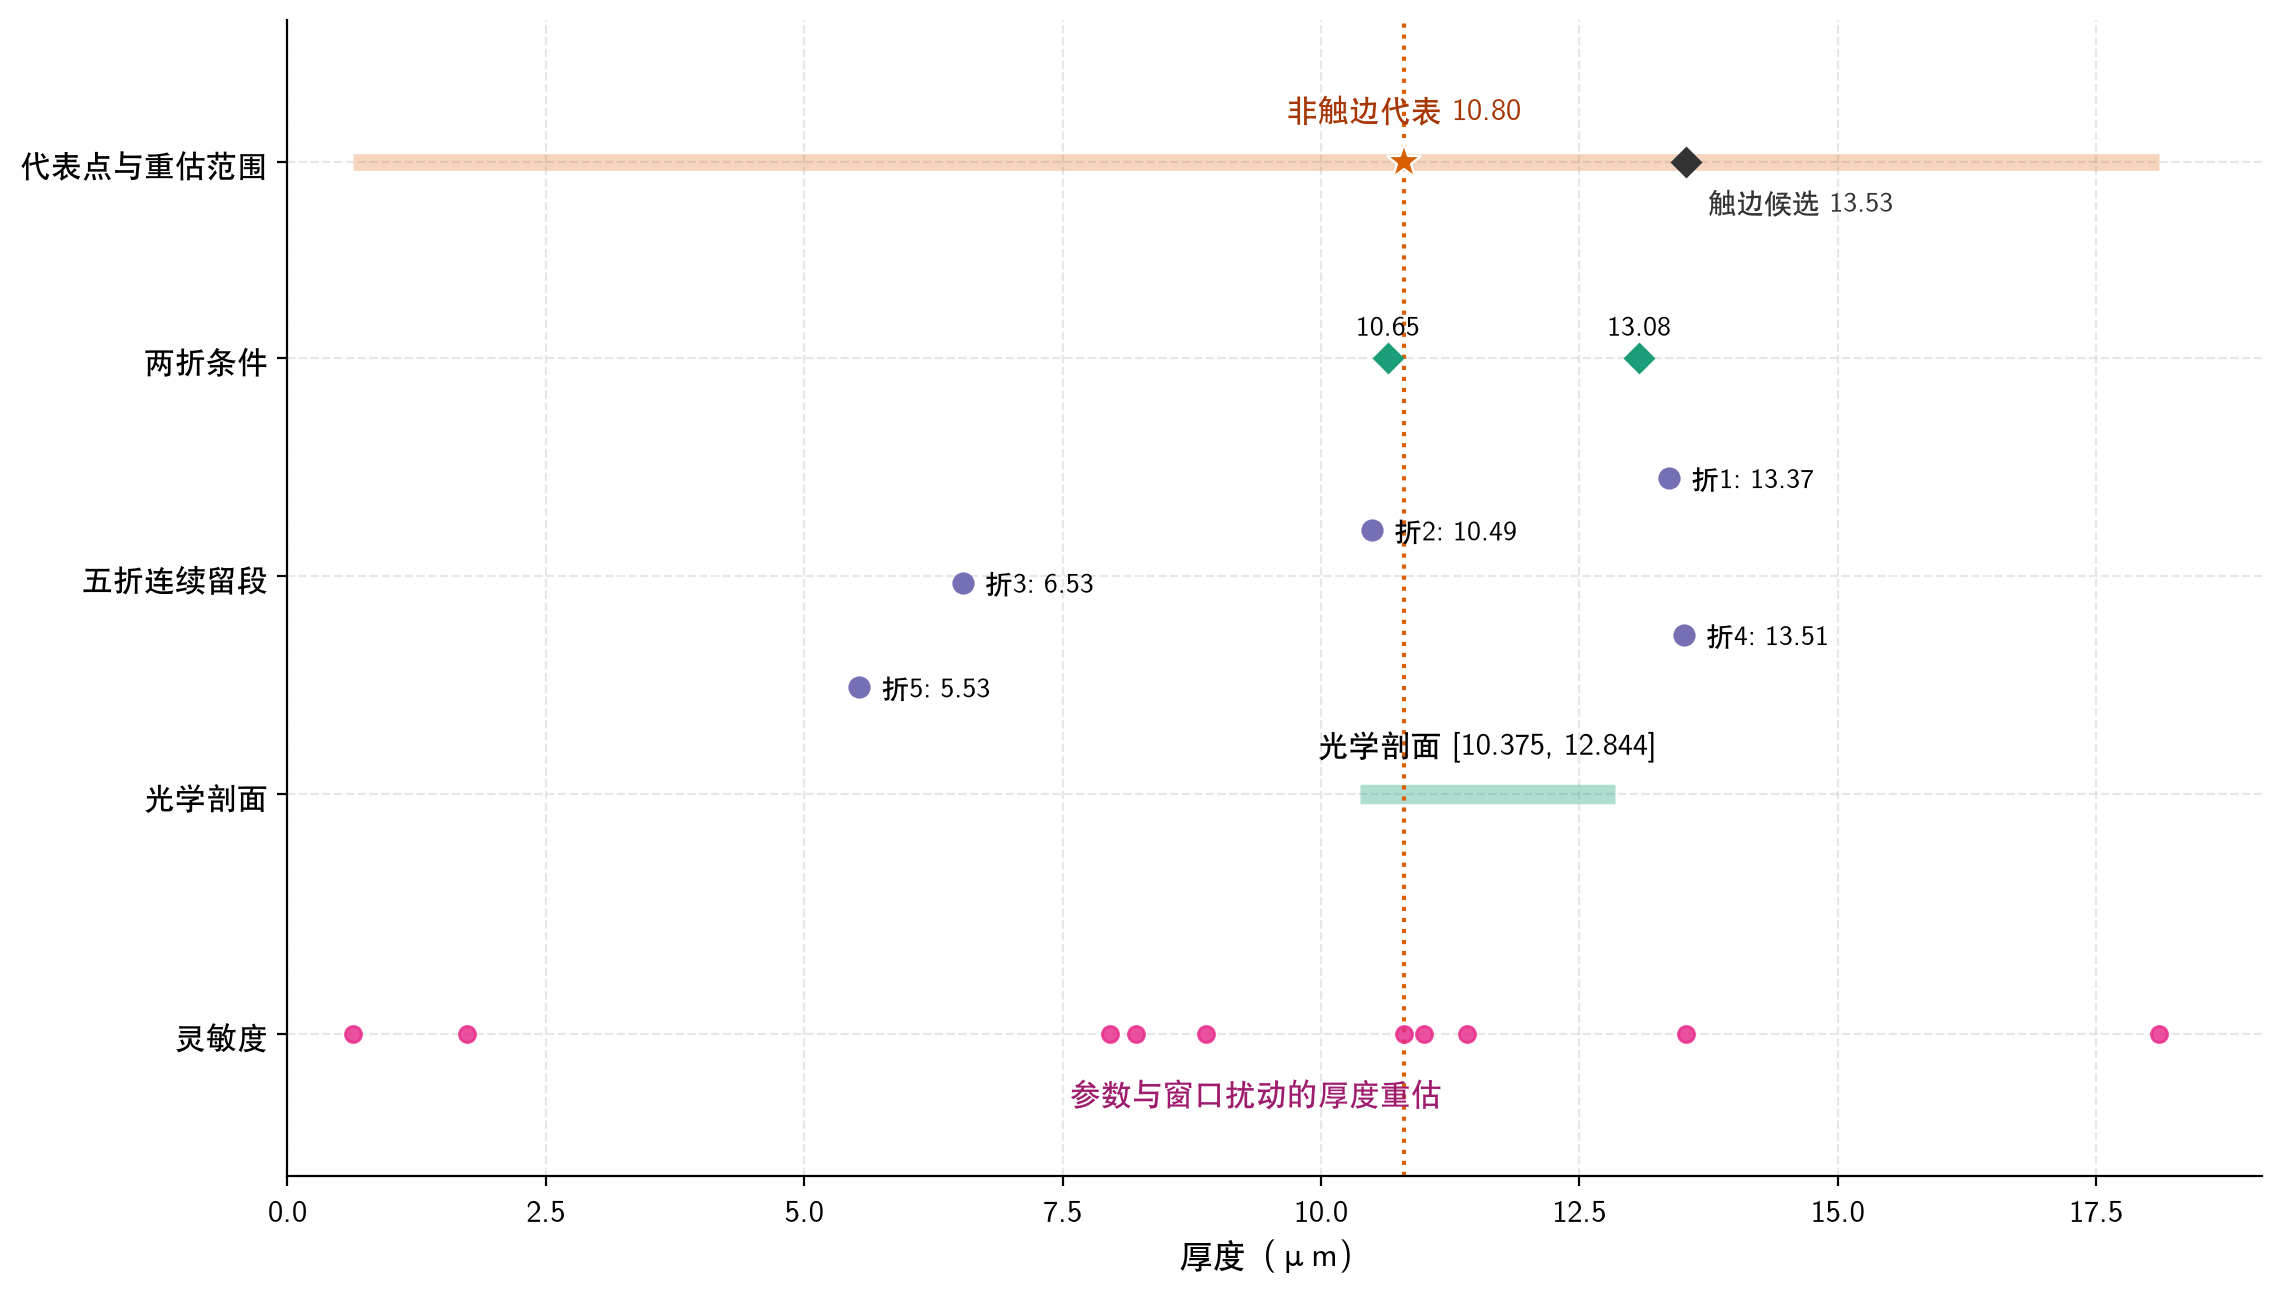
\includegraphics[width=0.8\textwidth,height=72.5mm,keepaspectratio]{../求解/问题2/图片/碳化硅厚度随假设变化.png}
  \caption{碳化硅厚度随切分和光学设置变化}
  \label{fig:q2-thickness}
\end{figure}

厚度分支虽随区段移动，条纹项仍增加了对留出光谱的解释力。正式连续留段标准化均方根误差为$1.2074$，低于二次趋势基线的$1.4404$，相对改善$16.17\%$；两项误差均无量纲，表示反射率预测误差相对于训练残差尺度的大小，按测试块等权平均。图\ref{fig:q2-residual}并列整体预测与局部残差，展示条纹拟合的总体优势和仍有偏差的波数区段。
% src:求解/问题2/结果/验证.json:正式主方法分数_连续留段标准化均方根误差;正式二次趋势基线分数_连续留段标准化均方根误差;正式主方法相对正式二次趋势改善_百分比;主指标含义

% 图10
\begin{figure}[!htb]
  \centering
  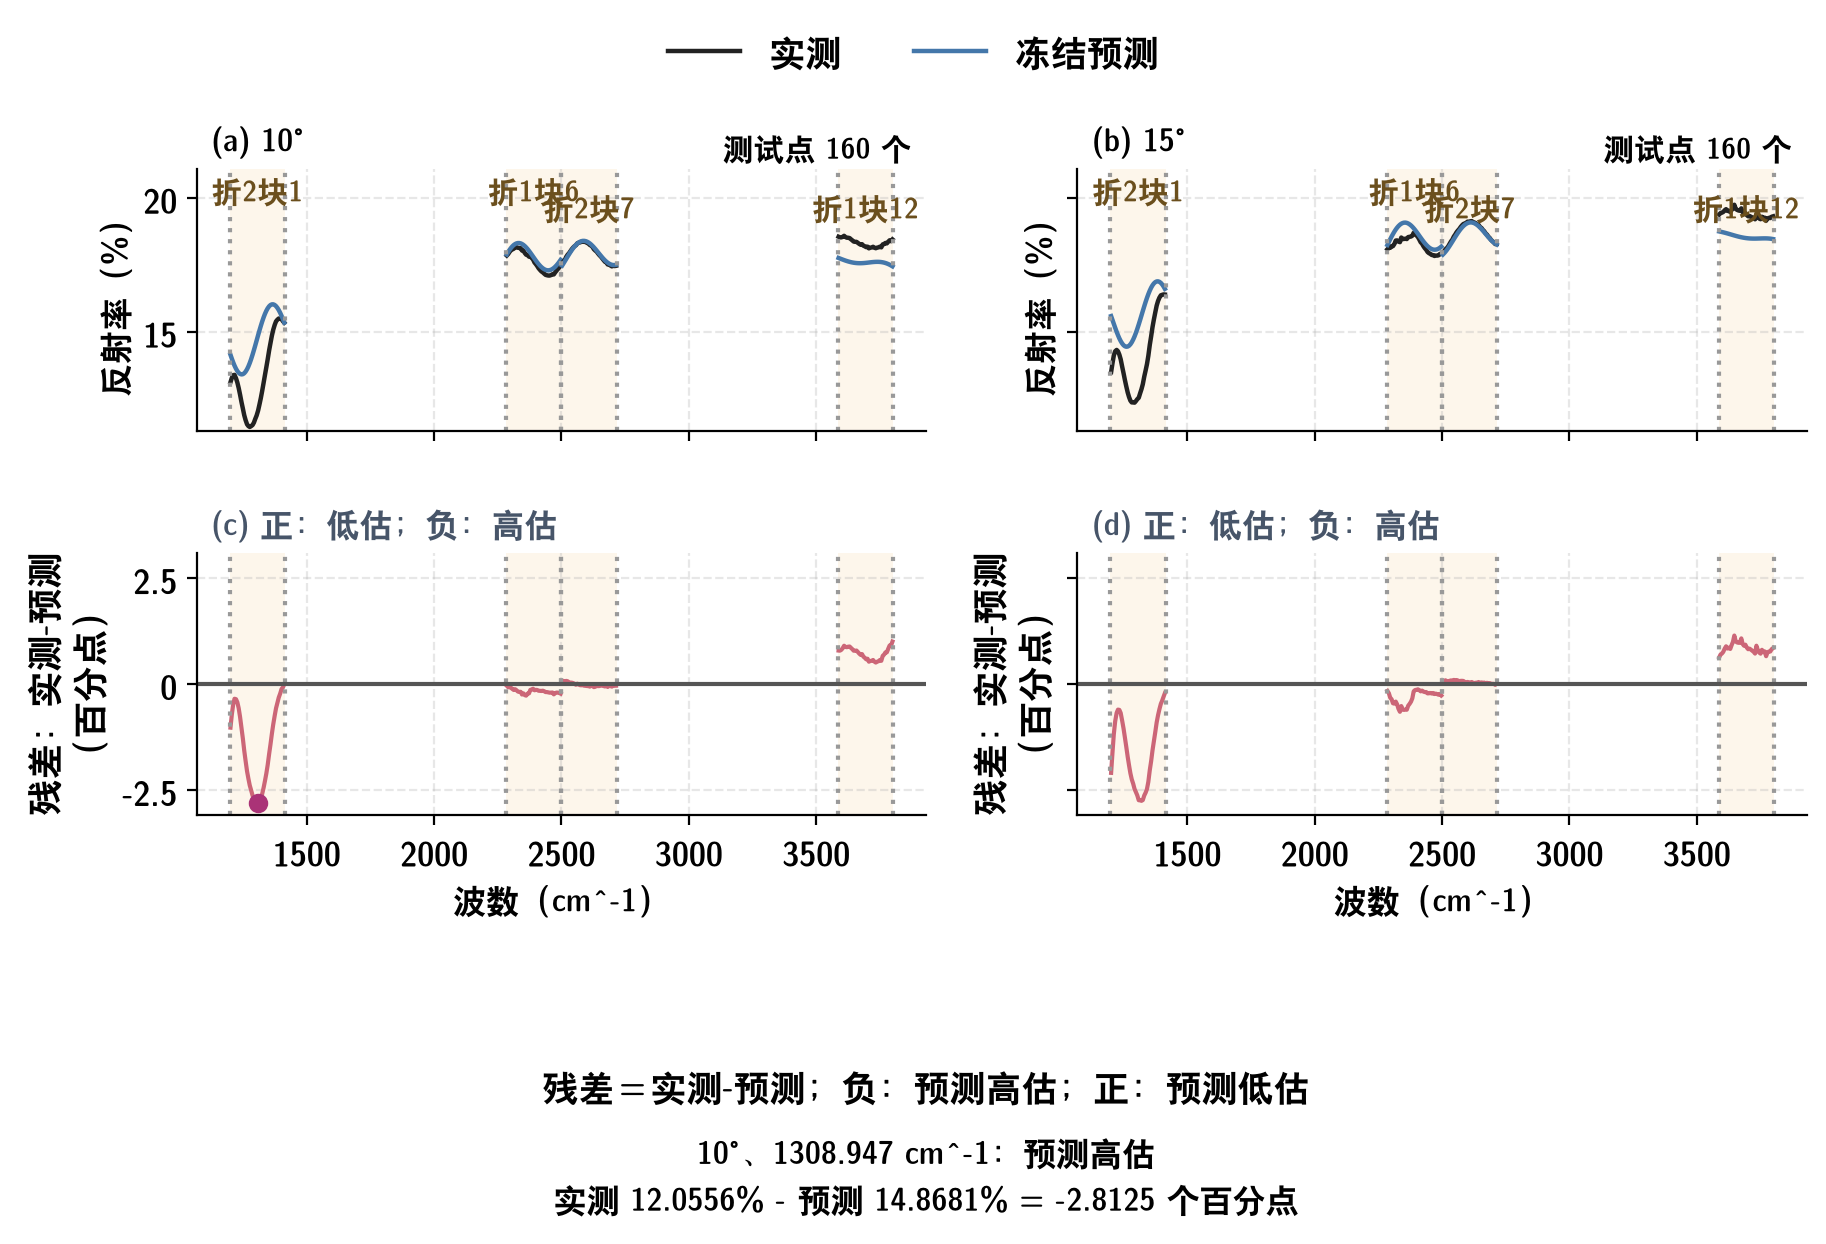
\includegraphics[width=0.96\textwidth]{../求解/问题2/图片/双角拟合残差显示局部偏差.png}
  \caption{双角光谱预测显示局部残差}
  \label{fig:q2-residual}
\end{figure}

局部偏差也曾改变区间的解释。最初把经验区间称为名义$90\%$区间时，连续测试块覆盖率仅为$50.63\%$；这次核对促使区间改用固定经验分位描述，并单独报告留出观测实际落入区间的比例。
% src:交接/实验记录.json:506.尝试;506.现象;506.决定

当前反射率区间以校准块绝对残差的$75\%$经验分位作为对称半宽，即将校准偏差由小到大排列，取该位置的偏差加在预测值两侧；测试经验覆盖率为$49.06\%$。图\ref{fig:q2-coverage}以校准分位为参照线，分块偏离说明校准段的误差宽度没有充分容纳测试段的偏差。
% src:求解/问题2/结果/区间覆盖.json:构造方法;校准经验分位点;测试经验覆盖率;覆盖解释

% 图14
\begin{figure}[!htb]
  \centering
  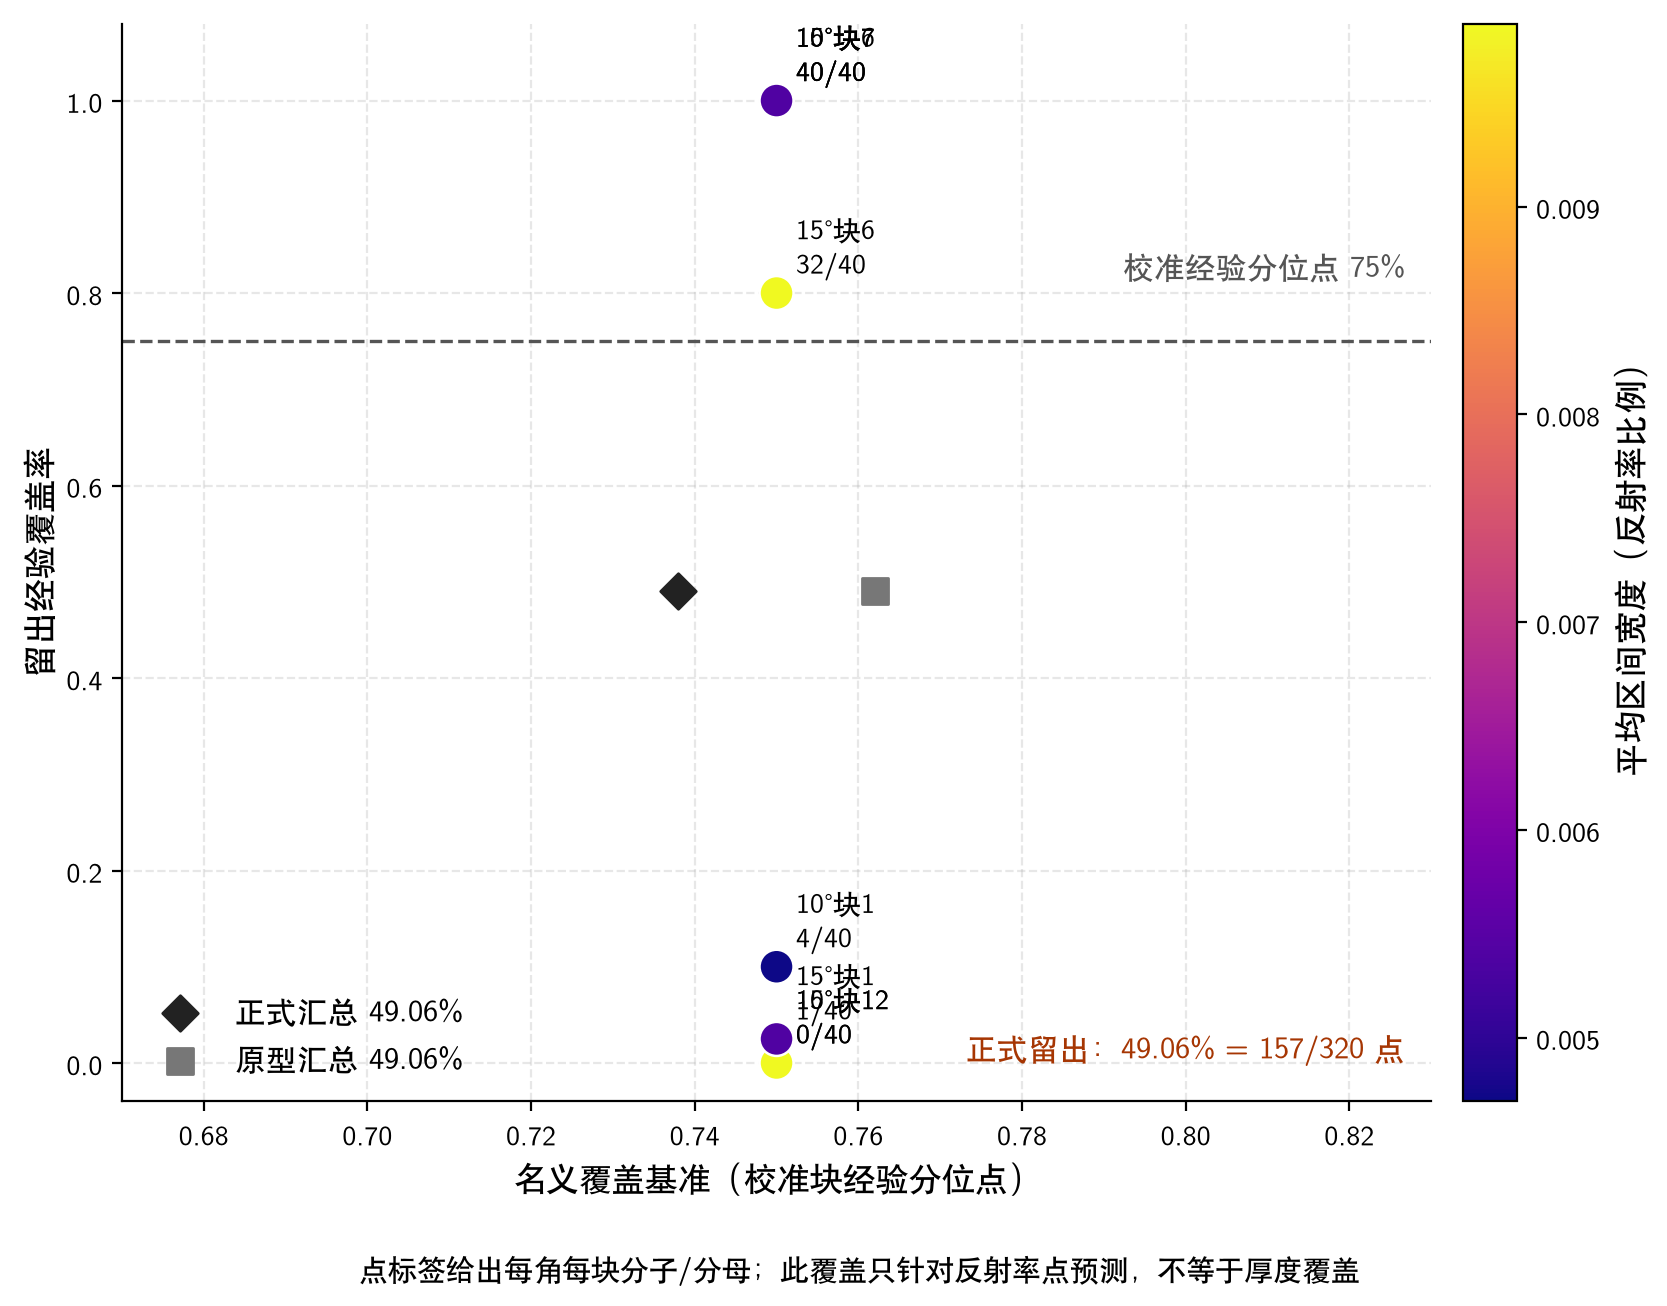
\includegraphics[width=0.8\textwidth,height=100mm,keepaspectratio]{../求解/问题2/图片/预测覆盖揭示区间失配.png}
  \caption{留出反射率覆盖偏离校准分位水平}
  \label{fig:q2-coverage}
\end{figure}

覆盖缺口把注意力引向跨角度的局部偏差。双向留角度核对固定每折共享厚度、色散及来源角相位，只在目标角训练点重估低阶基线与幅值；另一角的偏差便无法再靠自由调整厚度吸收。误差最大的测试块在正、反方向分别达到$3.457$和$2.965$，均无量纲，图\ref{fig:q2-angle}与表\ref{tab:q2-results}保留了其余块的差别。
% src:求解/问题2/结果/验证.json:双向留角度冻结诊断.4;双向留角度冻结诊断.6

% 图12


双向核对检验同片参数跨角度解释谱形的能力，碳化硅的同片拟合厚度为$10.80\ \mu\mathrm{m}$，厚度重估范围为$0.64$--$18.11\ \mu\mathrm{m}$。本问置信等级为低：五折厚度随切分明显变化，反射率测试覆盖不足，灵敏度情景形成较宽的厚度重估范围。该范围汇集光学假设下的重估结果，不是概率区间，反射率覆盖率也不是厚度覆盖率，绝对厚度仍需光学标定或标准厚度样片核对。问题三据此保留两束模型基准，检验更高阶往返是否足以改变这块晶圆的厚度判断。
% src:求解/问题2/结果/厚度结果.json:同片最佳厚度_微米;条件区间_微米
% src:交接/结果声明_问题2.json:置信.等级;置信.理由
